\section{Systembeskrivelse}
Det ønskes at udvikle et system, der har til formål at støtte musklerne omkring knæleddet hos ALS-patienter under udførelse af en squat-øvelse. 
Dette gøres for at aflaste patienterne med henblik på at udsætte brug af kørestol. 
Systemet skal kunne opsamle muskelsignaler fra rectus femoris og måle vinklen over knæet. 
Disse signaler skal behandles således, at de kan omsættes til signaler, så en prototype af et exoskelet kan udføre en tilsvarende bevægelse. 

Systemet har yderligere til formål at have mulighed for anvendelse i forskellige stadier af ALS. 
Ligeledes skal systemet være sikkert at anvende, hvortil sikkerhedsforanstaltninger er beskrevet i \autoref{sec:brugersikkerhed}. Derudover skal systemet ikke været til gene for brugeren, hvoraf systemet skal være trådløst og batteridrevet. %hvorfor trådløs kommunikation anvendes. Herudover skal systemet være batteridrevet, for at undgå en tilkobling til elnettet. Sikkerheden ses yderligere beskrevet i \autoref{sec:brugersikkerhed}. 
%Dette gør ligeledes systemet kompakt og mobilt. Hvis batterierne ikke kan levere nok strøm til, at systemet vil virke optimalt, skal dette indikeres. 
Da systemet ønskes at fungere i realtid, anses en forsinkelse på maksimum $100~ms$ som værende acceptabel. 

\subsection{Overordnet krav til systemet}  \label{sec:overordnet_krav}
\begin{itemize}
\item Systemet skal registrere muskelaktivitet fra rectus femoris 
\item Systemet skal måle vinklen over knæet
\item Systemet skal reagere på kroppens bevægelse under en squat-øvelse, således det vil kunne benyttes til en prototype af et exoskelet
\item Systemet skal være sikkert og ikke til gene for brugeren 
\item Systemet skal kunne overføre data trådløst til en computer
\item Systemet skal være batteridrevet
%\item Systemet skal kunne indikere, hvis der ikke er strøm nok til at virke optimalt
\item Systemet skal have en maksimal forsinkelse af hele systemet på $100~ms$
%\item Systemet skal kunne ende ud i en prototype af et exoskelet
\end{itemize}


\subsection{Blokdiagram} \label{sec:blokdiagram} 
\begin{figure}[H]
\centering
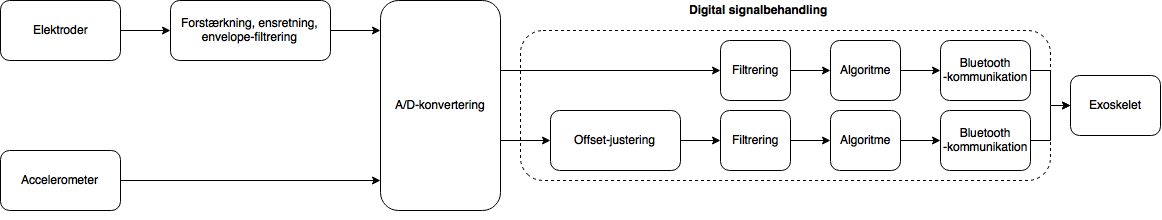
\includegraphics[width=1\textwidth]{figures/blokdiagram.png}
\caption{Systemets opbygning.}
\label{fig:blokdiagram}
\end{figure}

\noindent
Opbygningen af systemet fremgår af \autoref{fig:blokdiagram}. Der anvendes elektroder og accelerometre til at opsamle signaler. 
For at registrere muskelaktivitet anvendes elektroder, hertil ønskes det at forstærke, filtrere og ensrette muskelsignalet, der opsamles. 
Derudover anvendes accelerometre som en sensor.
De opsamlede signaler A/D-koverteres og sendes herefter videre til den digitale del af systemet, hvor en offsetjustering af accelerometer data, filtrering, algoritme samt trådløs kommunikation finder sted. 
Den digitale del skal bestå af et Bluetooth Low Energy Pioneer kit (CY8CKIT-042-BLE), som opfanger signalerne via elektroder og accelerometre. 
Herefter skal disse overføres trådløst til en computer, således en visualisering i MATLAB kan forekomme.
